\usetikzlibrary{arrows.meta,calc}
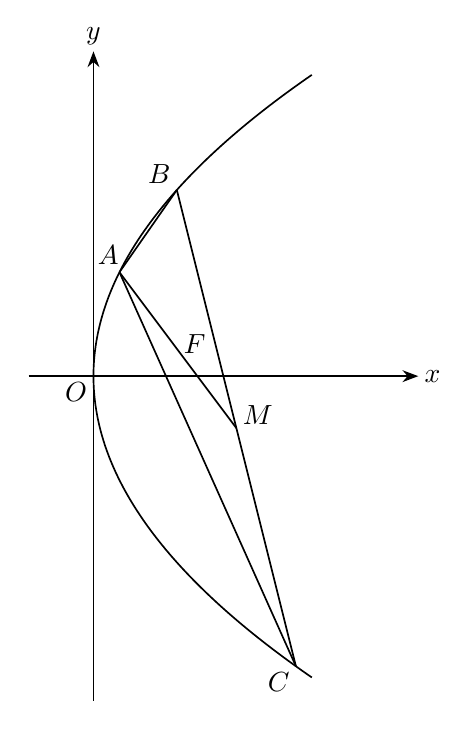
\begin{tikzpicture}[x=1cm,y=1cm,line width=.6pt,font=\normalsize,>=Stealth]
\coordinate (O) at (0,0);
\coordinate (A) at (0.33,1.32);
\coordinate (B) at (1.0589,2.3645);
\coordinate (C) at (2.5711,-3.6845);
\coordinate (F) at (1.32,0);
\coordinate (M) at (1.815,-0.66);
\coordinate (XMIN) at (-0.825,0);
\coordinate (XMAX) at (4.125,0);
\coordinate (YMIN) at (0,-4.125);
\coordinate (YMAX) at (0,4.125);
\draw[->] (XMIN) -- (XMAX);
\draw[->] (YMIN) -- (YMAX);
\draw[line width=.6pt] plot[domain=-23.19:23.19,samples=161] ({0.165*(\x*\x)/32},{0.165*\x});
\draw (A) -- (B);
\draw (B) -- (C);
\draw (A) -- (C);
\draw (A) -- (M);
\node[anchor=south east,inner sep=0pt] at (0.33,1.4082) {$A$};
\node[anchor=south east,inner sep=0pt] at (0.9883,2.4351) {$B$};
\node[anchor=north east,inner sep=0pt] at (2.5005,-3.7551) {$C$};
\node[anchor=south,inner sep=0pt] at (1.2847,0.2822) {$F$};
\node[anchor=south west,inner sep=0pt] at (1.8856,-0.6247) {$M$};
\node[anchor=north east,inner sep=0pt] at (-0.0706,-0.0706) {$O$};
\node[anchor=west,inner sep=0pt] at (4.1956,0.0) {$x$};
\node[anchor=south,inner sep=0pt] at (0.0,4.1956) {$y$};
\end{tikzpicture}
